\documentclass[11pt]{article}

\usepackage{latexsym}
\usepackage{graphicx}
\usepackage{amssymb}
\usepackage{amsthm}
\usepackage{enumerate}
\usepackage{amsmath}
\usepackage{cancel}
\numberwithin{equation}{section}

\setlength{\evensidemargin}{.25in}
\setlength{\oddsidemargin}{-.25in}
\setlength{\topmargin}{-.75in}
\setlength{\textwidth}{6.5in}
\setlength{\textheight}{9.5in}
\newcommand{\due}{February 4th, 2016}
\newcommand{\HWnum}{2}
\newcommand{\grad}{\bold\nabla}
\newcommand{\vecE}{\vec{E}}
\newcommand{\scrptR}{\vec{\mathfrak{R}}}
\newcommand{\kapa}{\frac{1}{4\pi\epsilon_0}}
\newcommand{\emf}{\mathcal{E}}
\newcommand{\unit}[1]{\ensuremath{\, \mathrm{#1}}}
\newcommand{\real}{\textnormal{Re}}
\newcommand{\Erf}{\textnormal{Erf}}
\newcommand{\sech}{\textnormal{sech}}
\newcommand{\scrO}{\mathcal{O}}
\newcommand{\levi}{\widetilde{\epsilon}}
\newcommand{\partiald}[2]{\ensuremath{\frac{\partial{#1}}{\partial{#2}}}}
\newcommand{\norm}[2]{\langle{#1}|{#2}\rangle}
\newcommand{\inprod}[2]{\langle{#1}|{#2}\rangle}
\newcommand{\ket}[1]{|{#1}\rangle}
\newcommand{\bra}[1]{\langle{#1}|}





\begin{document}
\begin{titlepage}
\setlength{\topmargin}{1.5in}
\begin{center}
\Huge{Physics 3320} \\
\LARGE{Principles of Electricity and Magnetism II} \\
\Large{Professor Ana Maria Rey} \\[1cm]

\huge{Homework \#\HWnum}\\[0.5cm]

\large{Joe Becker} \\
\large{SID: 810-07-1484} \\
\large{\due} 

\end{center}

\end{titlepage}



\section{Problem \#1}
\begin{enumerate}[(1)]
\item For a system that consists of an ensemble of three-level systems where we have $N$ 
particles with fixed positions each with 3 levels of energy given by $0$ and $\pm\epsilon$.
This implies for a state with energy $E$ we have 
$$E = N_{+}\epsilon + N_{0}(0) + N_{-}(-\epsilon) = (N_{+} -  N_{-})\epsilon$$
Where the total number of particles is given by the sum
$$N = N_{+} + N_{0} + N_{-}$$
Using these two relation we are able to find the entropy, $S$, of a state with energy, $E$, by 
noting that the statistical weight, $\Gamma(N_{+},N_{-},N_{0},N)$, is the number of states
that have energy $E$ that is the number of ways to arrange $N_{+}$ particles out of $N$ and 
$N_{-}$ particles out of the remaining $N-N_{+}$ available particles. Mathematically this is
\begin{align*}
\Gamma(N_{+},N_{-},N_{0},N) &= {{N}\choose{N_{+}}}{{N-N_{+}}\choose{N_{-}}} \\
&= \frac{N!}{N_{+}!\cancel{(N-N_{+})!}}\frac{\cancel{(N-N_+)!}}{N_{-}!(N-N_{+}-N_{-})!}\\
&= \frac{N!}{N_{+}!N_{-}!N_{0}!}
\end{align*}
Note we used the relation that $N_0=N-N_+-N_-$. Now we can find the entropy of the state by
\begin{align*}
\frac{S}{k} &= \ln\left(\Gamma\right)\\
&= \ln\left( \frac{N!}{N_{+}!N_{-}!N_{0}!}\right)\\
&= \ln(N!) - \ln(N_+) - \ln(N_-) - \ln(N_0)\\
&= \ln\left(\sqrt{2\pi}N^{N+1/2}e^{N}\right) - \ln\left(\sqrt{2\pi}N_+^{N_++1/2}e^{N_+}\right)- \ln\left(\sqrt{2\pi}N_-^{N_-+1/2}e^{N_-}\right)- \ln\left(\sqrt{2\pi}N_0^{N_0+1/2}e^{N_0}\right)\\
&= N\ln(N) + N + \frac{1}{2}\ln(N) + \frac{1}{2}\ln(2\pi) - N_+\ln(N_+) - N_+ - \frac{1}{2}\ln(N_+) - \frac{1}{2}\ln(2\pi) \\
&\qquad - N_-\ln(N_-) - N_- - \frac{1}{2}\ln(N_-) - \frac{1}{2}\ln(2\pi) - N_0\ln(N_0) - N_0 - \frac{1}{2}\ln(N_0) - \frac{1}{2}\ln(2\pi) \\
&= N\ln(N) + \frac{1}{2}\ln(N) - N_+\ln(N_+) - \frac{1}{2}\ln(N_+) - N_-\ln(N_-) - \frac{1}{2}\ln(N_-) \\
&\qquad   - N_0\ln(N_0) - \frac{1}{2}\ln(N_0) + \cancel{N - (N_++N_-+N_0)} - \ln(2\pi) \\
&\approx N\ln(N) - N_+\ln(N_+) - N_-\ln(N_-) - N_0\ln(N_0) 
\end{align*}
Now we wish to find the number $N_0$ that maximizes $S$ for a fixed energy, $E$, and total
number of particles, $N$. To do this we write $N_+$ and $N_-$ in terms of $E$ and $N$ by
\begin{align*}
N_+ = \frac{1}{2}\left(N-N_0+\frac{E}{\epsilon}\right)\\
N_- = \frac{1}{2}\left(N-N_0-\frac{E}{\epsilon}\right)
\end{align*}
This allows us to write $S$ as
\begin{align*}
\frac{S}{k} &= N\ln(N) - \frac{1}{2}\left(N-N_0+\frac{E}{\epsilon}\right)\ln\left(\frac{1}{2}\left(N-N_0+\frac{E}{\epsilon}\right)\right)\\
&\qquad - \frac{1}{2}\left(N-N_0-\frac{E}{\epsilon}\right)\ln\left(\frac{1}{2}\left(N-N_0+\frac{E}{\epsilon}\right)\right) - N_0\ln(N_0) 
\end{align*}
And by differentiating with respect to $N_0$ we can maximize $S$ by
\begin{align*}
\frac{1}{k}\partiald{S}{N_0} = 0 &= -\frac{1}{2}\left(-\ln\left(\frac{1}{2}\left(N-N_0+\frac{E}{\epsilon}\right)\right) -\frac{1}{2}\frac{N-N_0+E/\epsilon}{N-N_0+E/\epsilon}\right)\\
&\qquad -\frac{1}{2}\left(-\ln\left(\frac{1}{2}\left(N-N_0-\frac{E}{\epsilon}\right)\right) -\frac{1}{2}\frac{N-N_0-E/\epsilon}{N-N_0-E/\epsilon}\right)\\
&\qquad - \ln(N_0) - \frac{N_0}{N_0}\\
&\Downarrow\\
2\ln(2N_0) &= \ln\left(N-N_0-\frac{E}{\epsilon}\right) + \ln\left(N-N_0+\frac{E}{\epsilon}\right)\\
&\Downarrow\\
4N_0^2 &= \left(N-N_0-\frac{E}{\epsilon}\right)\left(N-N_0+\frac{E}{\epsilon}\right)\\
&\Downarrow\\
N_0 &= \frac{1}{3}\left(-N+\sqrt{4N^2-3\frac{E^2}{\epsilon^2}}\right)
\end{align*}
Note we took the positive solution of the quadratic as we require $N_0$ to be positive. Also
note that the relation $N\epsilon>\sqrt{3}E/2$ always holds due to the fact that the maximum 
possible energy is $N\epsilon$ which will always be larger than $E$.

\item We can use the partition function to repeat the calculation in part (1) by stating 
for a single particle we have
\begin{align*}
Z_{1} = \sum_{i=-1}^{1}e^{-\beta\epsilon_{i}} &= e^{-\beta(-\epsilon)} + e^{-\beta(0)} + e^{-\beta\epsilon}\\
&= 1 + e^{\beta\epsilon} + e^{-\beta(0)} + e^{-\beta\epsilon}\\
&= 1 + 2\cosh(\beta\epsilon)
\end{align*}
Where $\beta = 1/kT$. We note that the $N$ particles are independent so the total partition 
function is
$$Z_N = (1 + 2\cosh(\beta\epsilon))^N$$
using $Z_N$ we are able to calculate the entropy by
\begin{align*}
\frac{S}{k} &= \partiald{}{T}\left(\frac{}{}T\ln(Z_N)\right)\\
&= N\ln(1+2\cosh(\epsilon/kT)) + T\partiald{}{T}\left(N\ln(1+2\cosh(\epsilon/kT))\right)\\
&= N\ln(1+2\cosh(\epsilon/kT)) + NT\left(\frac{2\sinh(\epsilon/kT)}{1+2\cosh(\epsilon/kT)}\frac{-\epsilon}{kT^2}\right)\\
&= N\left(\ln(1+2\cosh(\epsilon/kT)) - \frac{2\epsilon}{kT}\frac{\sinh(\epsilon/kT)}{1+2\cosh(\epsilon/kT)}\right)
\end{align*}

\item Note that the result from part (2) we recover entropy as a function of $T$ given by
$$S(T) = Nk\left(\ln(1+2\cosh(\epsilon/kT)) - \frac{2\epsilon}{kT}\frac{\sinh(\epsilon/kT)}{1+2\cosh(\epsilon/kT)}\right)$$

\item We can find the dependence of energy on temperature by taking the derivative of the
partition function with respect to $\beta$ by
\begin{align*}
\average{E} &= -\partiald{}{\beta}\ln(Z_N)\\
&= -N\partiald{}{\beta}\ln(1+2\cosh(\beta\epsilon))\\
&= -\frac{2N\epsilon\sinh(\beta\epsilon)}{1+2\cosh(\beta\epsilon)}\\
\end{align*}
Which if we write in terms of $T$ we have
$$E(T) = -\frac{2N\epsilon\sinh(\epsilon/kT)}{1+2\cosh(\epsilon/kT)}$$
noting that the hyperbolic cosine function is always positive we see that the temperature at
which $E=0$ is given by
\begin{align*}
0 &= \sinh(\epsilon/kT)\\
&\Downarrow\\
0 &= \frac{\epsilon}{kT}
\end{align*}
This holds true when $kT>>\epsilon$ or when the temperature is much larger than the internal
energy levels of this system. This allows the states to be equally distributed between the 
$+$ and $-$ states which is when $E=0$. We note for the energy to be positive we need to have
$\sinh(\epsilon/kT)$ be negative as all other terms must be positive. This only occurs when
$\epsilon/kT$ is negative which implies that for $E>0$ we must have $T<0$. This makes sense 
as the state where $E>0$ has a heavily populated $N_+$ which corresponds to a highly unstable
state.

\item We calculate the specific heat by defining $m$ as the mass of a particle. It follows 
that
\begin{align*}
c = \frac{C}{m} = \frac{T}{m}\partiald{S}{T} &= \frac{NkT}{m}\partiald{}{T}\left(\left(\ln(1+2\cosh(\epsilon/kT)) - \frac{2\epsilon}{kT}\frac{\sinh(\epsilon/kT)}{1+2\cosh(\epsilon/kT)}\right)\right)\\
&= \frac{2N\epsilon^2}{mkT^2}\frac{2+\cosh(\epsilon/kT)}{(1+2\cosh(\epsilon/kT))^2}
\end{align*}
\begin{figure}
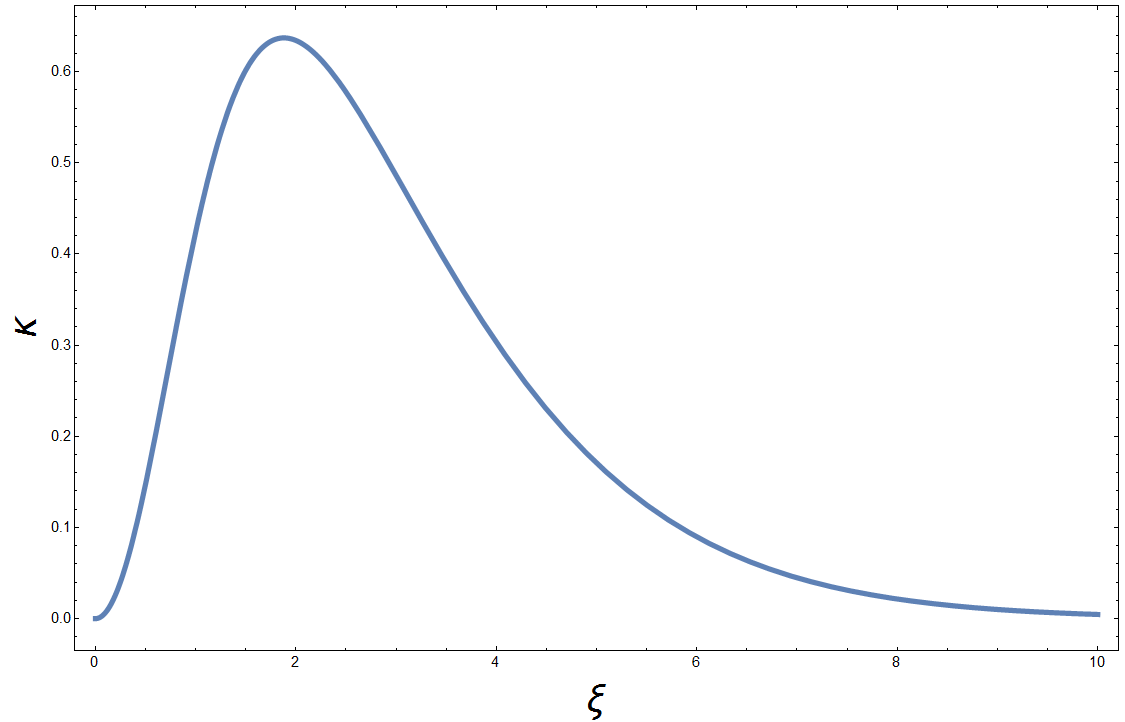
\includegraphics[width=1.0\textwidth]{Plot.png}
\caption{Plot of specific heat verses temperature using the unit-less quantities $\kappa$ and $\xi$.}
\label{Plot}
\end{figure}
We plot the function 
$$\kappa(\xi) = 2\xi^2\frac{2+\cosh\xi}{(1+2\cosh\xi)^2}$$
in figure \ref{Plot} using the unit-less quantities $K$ and $\xi$ defined as
$$\kappa \equiv \frac{cm}{Nk},\qquad \xi \equiv \frac{\epsilon}{kT}$$
Note that in the two limiting cases of large temperatures, $\xi=0$, and large energy steps 
relative to $kT$, $\xi>>1$ we are at a specific heat of zero. An we are at a max at $\xi=2$ 
or when $kT=2\epsilon$.

\item We can calculate the fluctuations in the energy verses the temperature by taking the
derivative of $E$ with respect to $T$. Using the relation we found in part (4) we see
\begin{align*}
\partiald{E}{T} &= \partiald{}{T}\left(-\frac{2N\epsilon\sinh(\epsilon/kT)}{1+2\cosh(\epsilon/kT)}\right)\\
&= \frac{2N\epsilon^2}{kT^2}\frac{2+\cosh(\epsilon/kT)}{(1+2\cosh(\epsilon/kT))^2}
\end{align*}
We note that this expression is the exact same as the expression for the heat capacity of the
system. Note the loss of the factor of $m$. This make sense as the system is not dependent on
the quantities of pressure and volume with implies that no work is done on or by the system.
Therefore the total change in energy comes from the change in heat. This is related to the
change in temperature by the heat capacity.
\end{enumerate}
\end{document}

